Das UI und UX Design war bei der Entwicklung des Kundenmanagement Tool ebenfalls ein wichtiger Teil. Einer unserer ersten Schritte war es ein Grundgerüst zu bauen, in welchem wir das UX Design einarbeiten. Für das UI Design wurden daraufhin einige Grundlagen wie Farben oder die verwendete Schriftart festgelegt. Der letzte Schritt vor der Implementierung war es einige Grundelement zu definieren. Dazu zählte beispielsweise das Design eines Buttons, der Navigation oder auch des Contents.

Bei unserem Produkt war das UX-Design am wichtigsten. Die Mitarbeiter vom Planfred Support arbeiten am Tag hauptsächlich mit diesem Produkt, dadurch sollte die Verwendung so intuitiv und einfach wie möglich sein.

\textbf{Beispiel:}
\newline
Wir haben uns im Bezug auf die Navigation für eine seitliche Navigationsbar entschieden:

\begin{figure}[h!]
    \centering
    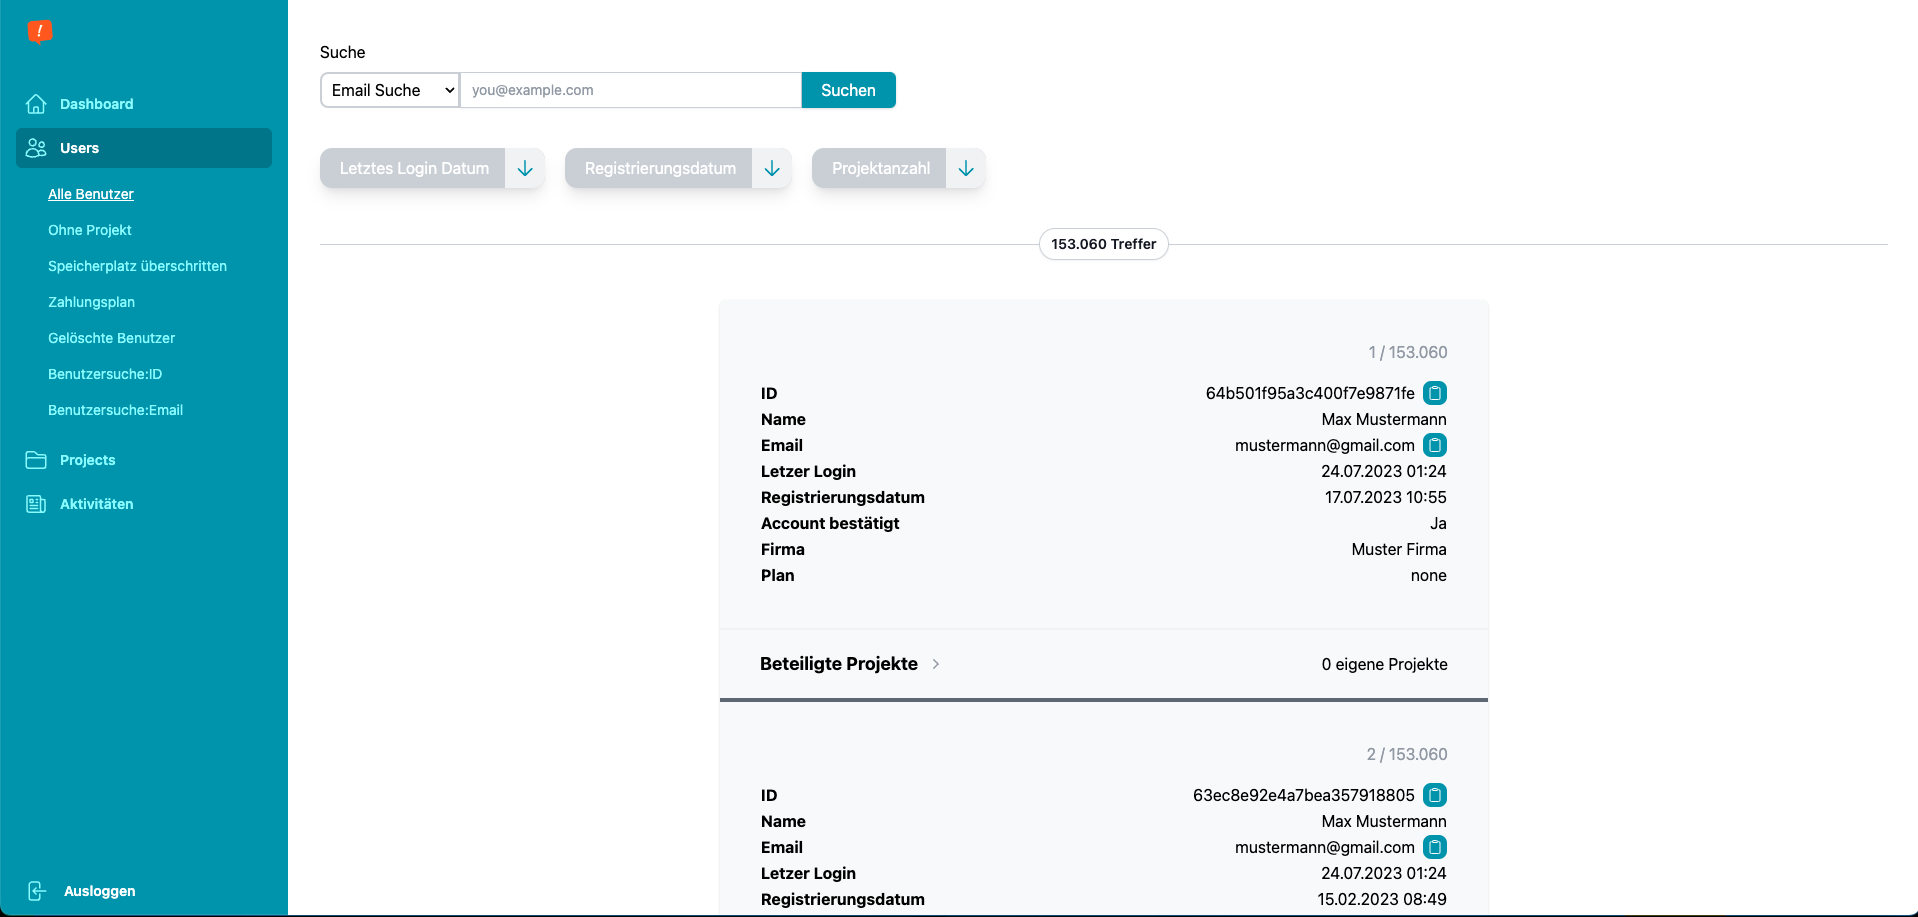
\includegraphics[width=1\textwidth]{pics/planfred-ui-ux-example.png}
    \caption{Planfred Design Beispiel}
    \label{fig:mesh1}
\end{figure}

Grund für diese Entscheidung sind die vielen Unterpunkte. Grundlegend gibt es 4 Hauptseiten. Dabei gibt es jedoch noch zahlreiche Unterseiten, welche jedoch nur angezeigt werden, wenn die jeweilige Hauptseite ausgewählt ist. Das sorgt für eine bessere Übersicht und verwirrt die Benutzer:innen nicht unnötig. 